\appendixsection{Finite element method (FEM)}\labelappendixframe{frame:appfem}

\begin{appendixframe}{Construction of the unknown vector}\labelappendixframe{frame:basis}

	Considering $(\phi_i)_{i=1}^{N_u}$, $(\psi_j)_{j=1}^{N_p}$ and $(\eta_k)_{k=1}^{N_T}$ the basis functions of the finite element spaces $V_h^{\, 0}$, $Q_h$ and $W_h$ respectively, we can write the discrete solutions as:
	\begin{equation*}
		\bm{u}_h(\bm{x}) = \sum_{i=1}^{N_u} \begin{pmatrix}
			u_i \\
			v_i
		\end{pmatrix} \phi_i(\bm{x}), \quad p_h(\bm{x}) = \sum_{j=1}^{N_p} p_j \psi_j(\bm{x}) \quad \text{and} \quad T_h(\bm{x}) = \sum_{k=1}^{N_T} T_k \eta_k(\bm{x}),
	\end{equation*}	
	with the unknown vectors for velocity, pressure and temperature defined by

	\vspace{-5pt}
	$$\vec{u} = \big(u_i\big)_{i=1}^{N_u} \in \mathbb{R}^{N_u}, \quad \vec{v} = \big(v_i\big)_{i=1}^{N_u} \in \mathbb{R}^{N_u},$$
	$$\vec{p} = \big(p_j\big)_{j=1}^{N_p} \in \mathbb{R}^{N_p} \; \text{ and } \; \vec{T} = \big(T_k\big)_{k=1}^{N_T} \in \mathbb{R}^{N_T}.$$

	\vspace{5pt}
	Considering $N_h = 2N_u + N_p + N_T$, we can define the global vector of unknowns as:
	\begin{equation*}
		\vec{U} = \big(\vec{u}, \vec{v}, \vec{p}, \vec{T}) \in \mathbb{R}^{N_h}.
	\end{equation*}
	and $F:\mathbb{R}^{N_h} \to \mathbb{R}^{N_h}$ the nonlinear operator associated to the weak formulation \eqref{eq:weak_pb}.
\end{appendixframe}

\appendixsection{PINN Initialization / Additive approach}\labelappendixframe{frame:comp}


\begin{appendixframe}{Comparison of the 2 approaches}
	Taking $U_\theta$ and $C_h^+$ in the same space, we have :
	$$F_\theta(\vec{C})=F(\vec{U}_\theta+\vec{C}),$$
	with $\vec{C}$ the correction vector and $\vec{U}_\theta$ the PINN vector (PINN evaluation at the dofs), both of size $N_h$.

	The first iteration of the additive approach :
	$$ F_\theta(\vec{C}^{(0)}) + F_\theta'(\vec{C}^{(0)}) \delta^{(1)} = 0 $$
	becomes (as $C^{(0)}=0$) :
	$$F(\vec{U}_\theta) + F'(\vec{U}_\theta)\delta^{(1)}=0,$$
	which is equivalent as the standard method with the PINN initialization.
\end{appendixframe}

%% AUTRES

\appendixsection{Results - Linear problem}\labelappendixframe{frame:linear}

\begin{appendixframe}{Problem considered} 
	\textbf{Problem statement:} Consider the Poisson problem with Dirichlet BC:
	\vspace{-5pt}
	\begin{equation*}
		\left\{
		\begin{aligned}
			-\Delta u & = f, \; &  & \text{in } \; \Omega \times \mathcal{M}, \\
			u         & =0, \;  &  & \text{on } \; \partial\Omega \times \mathcal{M},
		\end{aligned}
		\right.
		% \label{eq:Lap2D}\tag{$\mathcal{P}$}
	\end{equation*}

	\vspace{-5pt}
	with $\Omega=[-0.5 \pi, 0.5 \pi]^2$ and $\mathcal{M}=[-0.5,0.5]^2$ ($p=2$ parameters).
		
	\vspace{8pt}
	\textbf{Analytical solution :}

	\vspace{-5pt}
	\begin{equation*}
		% \label{eq:analytical_solution_Lap2D}
		u(\bm{x},\bm{\mu})=\exp\left(-\frac{(x-\mu_1)^2+(y-\mu_2)^2}{2}\right)\sin(2 x)\sin(2 y).
	\end{equation*}

	\vspace{12pt}
	\textbf{PINN training:} MLP of 5 layers; LBFGs optimizer (5000 epochs). \\
	Imposing the Dirichlet BC exactly in the PINN with the levelset $\varphi$ defined by
	$$\varphi(\bm{x})=(x+0.5\pi)(x-0.5\pi)(y+0.5\pi)(y-0.5\pi).$$
	
	\small\vspace{4pt}
	Training time : less than 1 hour on a laptop GPU.
\end{appendixframe}

\begin{appendixframe}{Numerical results}
	\hspace{-5pt}\begin{minipage}[t]{0.46\linewidth}
		\textbf{Error estimates :} 1 set of parameters.
		$$\bm{\mu}^{(1)}=(0.05, 0.22) $$
		\vspace{-35pt}
		\begin{figure}[H]
			\cvgFEMCorrAlldeg{images/appendix/linear_results/cvg/FEM_case1_v1_param1.csv}{images/appendix/linear_results/cvg/Corr_case1_v1_param1.csv}{1e-10}
		\end{figure}
	\end{minipage} \qquad \small
	\begin{minipage}[t]{0.48\linewidth}
	\end{minipage}
\end{appendixframe}

\begin{appendixframe}{Numerical results}[noframenumbering]
	\hspace{-5pt}\begin{minipage}[t]{0.46\linewidth}
		\textbf{Error estimates :} 1  set of parameters.
		$$\bm{\mu}^{(1)}=(0.05, 0.22) $$
		\vspace{-35pt}
		\begin{figure}[H]
			\cvgFEMCorrAlldeg{images/appendix/linear_results/cvg/FEM_case1_v1_param1.csv}{images/appendix/linear_results/cvg/Corr_case1_v1_param1.csv}{1e-10}
		\end{figure}
	\end{minipage} \qquad \small
	\begin{minipage}[t]{0.48\linewidth}
		\textbf{Gains achieved :} $n_p=50$ sets of parameters.
		$$\mathcal{S}=\left\{\bm{\mu}^{(1)},\dots,\bm{\mu}^{(n_p)}\right\}$$
		\vspace{-15pt}
		\begin{table}[H]
			\gainstableallq{images/appendix/linear_results/gains/Tab_stats_case1_v1.csv}
		\end{table}

		\normalsize\centering\vspace{-20pt}
		$$N=20$$

		\vspace{-5pt}
		Gain : $\| u-u_h\|_{L^2} / \| u-u_h^+\|_{L^2}$ \\
		
		\small\vspace{8pt}
		Cartesian mesh : $N^2$ nodes.
	\end{minipage}
\end{appendixframe}

\begin{appendixframe}{Numerical results}[noframenumbering]
	\hspace{-5pt}\begin{minipage}[t]{0.46\linewidth}
		\textbf{Error estimates :} 1 set of parameters.
		$$\bm{\mu}^{(1)}=(0.05, 0.22) $$
		\vspace{-35pt}
		\begin{figure}[H]
			\cvgFEMCorrAlldegLine{images/appendix/linear_results/cvg/FEM_case1_v1_param1.csv}{images/appendix/linear_results/cvg/Corr_case1_v1_param1.csv}{1e-10}
		\end{figure}
	\end{minipage} \qquad \small
	\begin{minipage}[t]{0.48\linewidth}
		\textbf{$N_\text{dofs}$ required to reach the same error $e$ :}

		\vspace{10pt}
		\begin{table}[H]
			\centering
			\coststableallq{images/appendix/linear_results/costs/TabDoFs_case1_v1_param1.csv}
		\end{table}
	\end{minipage}
\end{appendixframe}

\appendixsection{Data-driven vs Physics-Informed training}\labelappendixframe{frame:datavspinns}

\begin{appendixframe}{Problem considered}
	\textbf{Problem statement:} Consider the Poisson problem in 1D with Dirichlet BC:
	\vspace{-5pt}
	\begin{equation*}
		\left\{
		\begin{aligned}
			-\partial_{xx} u & = f, \; &  & \text{in } \; \Omega \times \mathcal{M}, \\
			u         & = 0, \;  &  & \text{on } \; \partial\Omega \times \mathcal{M},
		\end{aligned}
		\right.
		% \label{eq:Lap2D}\tag{$\mathcal{P}$}
	\end{equation*}

	\vspace{-5pt}
	with $\Omega=[0,1]^2$ and $\mathcal{M}=[0,1]^3$ ($p=3$ parameters).
		
	\vspace{4pt}
	\textbf{Analytical solution :} $\quad u(x;\bm{\mu})=\mu_1\sin(2\pi x)+\mu_2\sin(4\pi x)+\mu_3\sin(6\pi x) \,.$

	\vspace{4pt}
	\textbf{Construction of two priors:} MLP of 6 layers; Adam optimizer (10000 epochs). \\
	Imposing the Dirichlet BC exactly in the PINN with $\varphi(x)=x(x-1)$.

	\begin{itemize}
		\item \textbf{Physics-informed training:} $N_\text{col}=5000$ collocation points.
		$$J_r(\theta) \simeq
			\frac{1}{N_\text{col}} \sum_{i=1}^{N_\text{col}} \big| \partial_{xx}u_\theta(\bm{x}_\text{col}^{(i)};\bm{\mu}_\text{col}^{(i)}\big) + f\big(\bm{x}_\text{col}^{(i)};\bm{\mu}_\text{col}^{(i)}\big) \big|^2.$$
	
		\item \textbf{Data-driven training:}  $N_\text{data}=5000$ data.
		$$J_\text{data}(\theta) =
		\frac{1}{N_\text{data}}
		\sum_{i=1}^{N_\text{data}} \big| u_\theta^\text{data}(\bm{x}_\text{data}^{(i)};\bm{\mu}_\text{data}^{(i)}) - u(\bm{x}_\text{data}^{(i)};\bm{\mu}_\text{data}^{(i)}) \big|^2.$$
	\end{itemize}
\end{appendixframe}

\begin{appendixframe}{Priors derivatives}
	\vspace{-10pt}
	$$\bm{\mu}^{(1)}=(0.3,0.2,0.1)$$
	\begin{figure}[ht!]
		\centering
		\rotatebox{90}{PINN}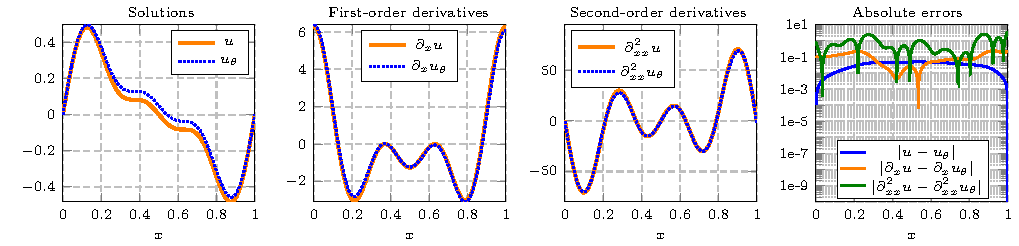
\includegraphics[width=0.95\linewidth]{images/appendix/datavspinns/standalone_solutions_and_errors_PINN.pdf}
	\end{figure}
	
	\begin{figure}[ht!]
		\centering
		\rotatebox{90}{Data}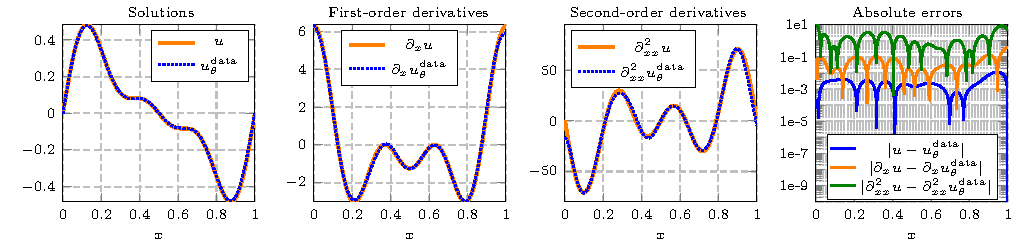
\includegraphics[width=0.95\linewidth]{images/appendix/datavspinns/standalone_solutions_and_errors_NN.pdf}
	\end{figure}
\end{appendixframe}

\begin{appendixframe}{Additive approach in $\mathbb{P}_1$}
	\vspace{-2pt}
	\textbf{1 set of parameters:} $\quad \bm{\mu}^{(1)}=(0.3,0.2,0.1)$
	
	\begin{table}[H]
		\centering
		\gainsbothNN{images/appendix/datavspinns/FEM_param1.csv}{images/appendix/datavspinns/compare_gains_param1.csv}
	\end{table}

	\vspace{6pt}
	\textbf{50 set of parameters:}

	\begin{table}[H]
		\centering
		\gainstableMult{images/appendix/datavspinns/Tab_stats_case1_degree1.csv}
	\end{table}

	\footnotesize
	$N$ : Nodes.
\end{appendixframe}